% (This file is included by thesis.tex; you do not latex it by itself.)
\chapter{Discussion}
All coding was done using R code and packages available in R. The code is available on \href{https://github.com/ShilpikaB/Prioritizing-Network-Properties-of-T-Cell-Receptors}{\textbf{GitHub}} for reference.
\section{Inferences from Real Data Analysis}\label{sec:realdat_ana}
Through our work we have compared and demonstrated the model performances using both the cross-validation and the permutation tuning techniques. Using the real data, the Group Lasso\_CV (Group Lasso using Cross-Validation) model was able to prioritize three of the network properties (feature blocks)  --- \lq Membership' (\# of Clusters), \lq Count\_PRE\_INFUSION', and \lq Count\_DOSE\_2'. The Group Plasso (Group Lasso using permutation tuning) model selected only two of the aforementioned network properties --- \lq Membership' (\# of Clusters) and \lq Count\_PRE\_INFUSION'. The difference in the output of the two models can be attributed to the characteristics of the permutation tuning of having lower false positives (\cite{permassisttune}Yang \textit{et al.}, 2020) in comparison to the cross-validation technique. Therefore, the Group Plasso model appears to be more stringent than Group Lasso\_CV in performing variable selection on the network feature blocks. When using Lasso\_CV (Lasso using Cross-Validation) and Plasso (Lasso using permutation tuning) both models selected the same set of network features as the top performing variables --- the max summary statistics for the TCR network properties \lq Count\_PRE\_INFUSION', \lq diam\_length', \lq eigen\_centrality', \lq centr\_eigen'. Exclusive Lasso (using only cross-validation) model reaffirmed the findings from Lasso\_CV and Plasso by selecting the same set of network features from their corresponding feature blocks. The expectation was to observe overlap in the variables selected using the Group Lasso models and the Lasso models. The only common network property that was selected across all the models was \lq Count\_PRE\_INFUSION'. The dissimilarity in the selected variables could be attributed to the small sample size. Therefore, we extended our analysis onto the simulated data to enhance and substantiate our findings.\par

\section{Model Performance Comparison} \label{sec:perf_measure}
Prior to performing simulation study on Group Lasso\_CV and Group Plasso models, we used two distinct set of true variables as references --- feature blocks selected using Group Lasso\_CV on the real data; feature blocks corresponding to the network features selected using Lasso\_CV on the real data. This was done to maximize the possibility of identifying the true significant network properties. When the true variables were sourced from the feature blocks selected using Group Lasso\_CV on the real data, both Group Lasso\_CV and Group Plasso were able to select the desired set of feature blocks --- \lq Membership' (\# of Clusters), \lq Count\_PRE\_INFUSION', and \lq Count\_DOSE\_2'. The noteworthy observation was that Group Plasso performed better than Group Lasso\_CV across all the performance measures. Refer \autoref{tab:grp_lasso_sim_study}. Similarly, when using the other set of true variables, Group Plasso consistently outperformed Group Lasso\_CV for most of the performance measures. Refer \autoref{tab:grp_lasso_vs_lasso_sim_study}. In case of Lasso\_CV and Plasso models, Plasso performed better than Lasso. Refer \autoref{tab:lasso_sim_study}. The Plasso model had a higher false discovery rate (FDR) than that of the Lasso\_CV model because the Lasso\_CV model, in some iterations, was selecting zero features and hence the FDR value was computed as zero for those iterations. Whereas, the Plasso model almost always selected non-zero number of features and hence had a higher FDR value. Across all the models it was observed that permutation assisted tuning gave the models much higher stability than cross-validation. Empirically, permutation tuning may be more robust, accurate, reliable, and consistent than cross-validation technique when performing variable selection. However, formal verification would be required to establish and to generalize the observation that the performance of permutation tuning is superior than cross-validation for all variable selection problems.\par 

\section{Significant TCR Network Properties and Features} \label{sec:add_features}
Referring to the output from \autoref{tab:grp_model_selected_variables}, we aggregate the list of group indexes (feature blocks) that were selected by both Group Lasso\_CV and Group Plasso models. Similarly, for  Lasso\_CV and Plasso models we collect the feature indexes that were selected by both the models. Refer \autoref{tab:lasso_selected_variables}. The \autoref{fig:newfeat} ties up the Group Indexes from the Group Lasso models and the Feature Indexes from the Lasso models to the indexes of their corresponding TCR network properties and features. We observe that the network properties selected by the Group Lasso models completely encompass the network features selected by the Lasso models. This aligns with our initial intuition that the different variable selection models should have certain degree of overlap among the selected variables. We finally conclude that the most significant TCR network properties deduced from the variable selection methods are --- Membership (\# of clusters), Count Pre-infusion, Count Dose 2, Diameter Length, Transitivity and Central Eigen. The top network features associated with these network properties are --- the count of Membership (\# of clusters), the max value of Count Pre-infusion,  the median and the mean values of Count Dose 2, the mean and the max of Diameter Length, the $Q_3$ value of Transitivity, and the max value of Central Eigen.\par

\begin{figure}[H]
\centering
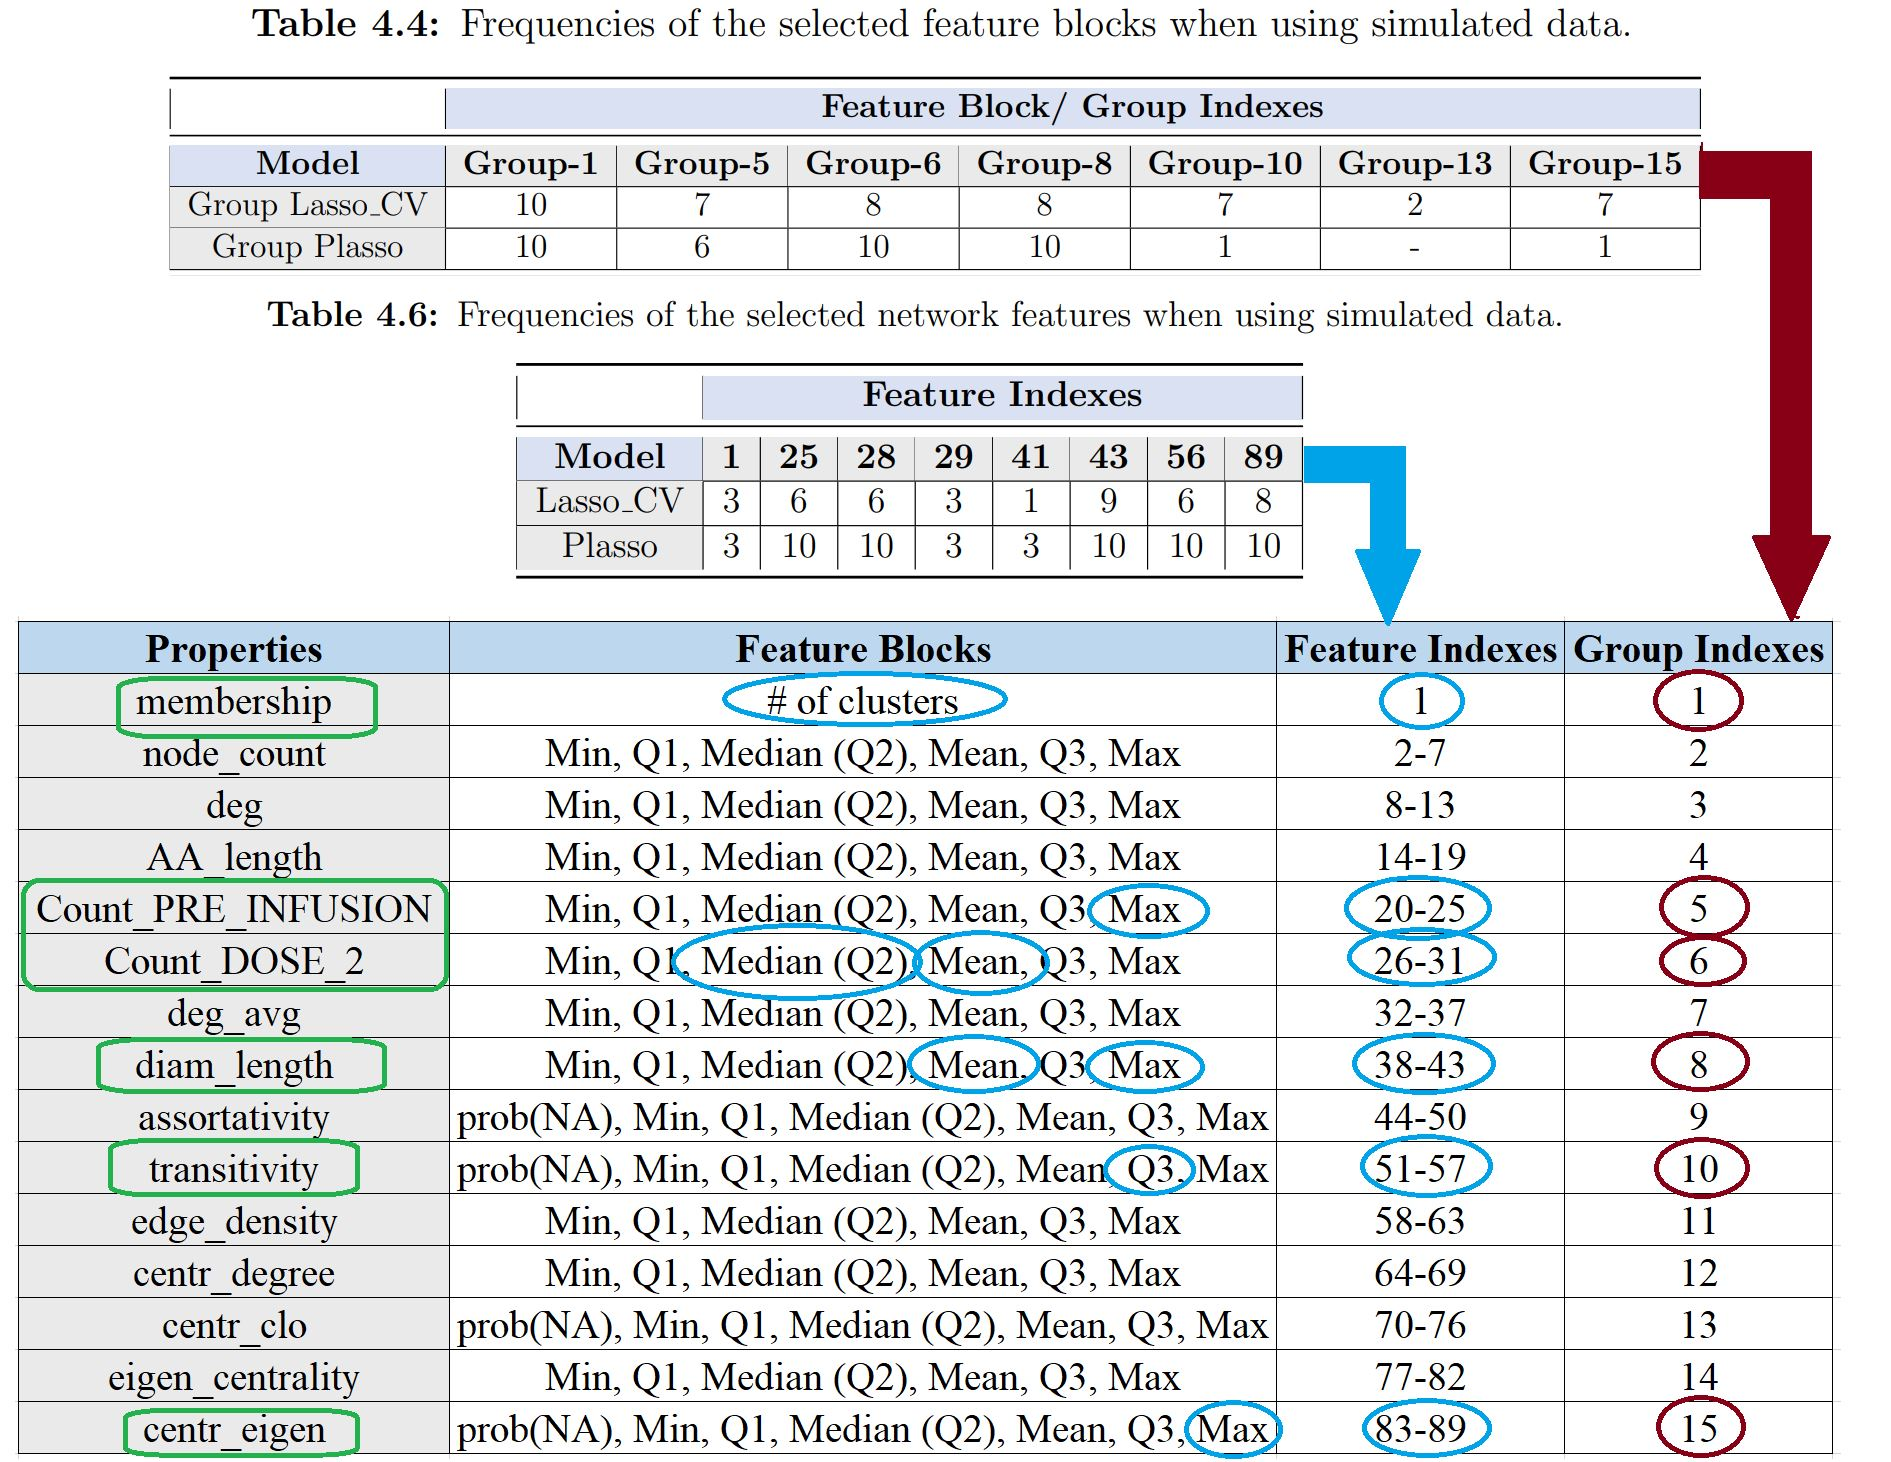
\includegraphics[scale=0.75]{NewFeatures_Simstudy.jpg}
\caption{Overlap in the features selected from Group Lasso models and Lasso models.}
\label{fig:newfeat}
\end{figure}